\begin{figure*}[t]
	\centering
	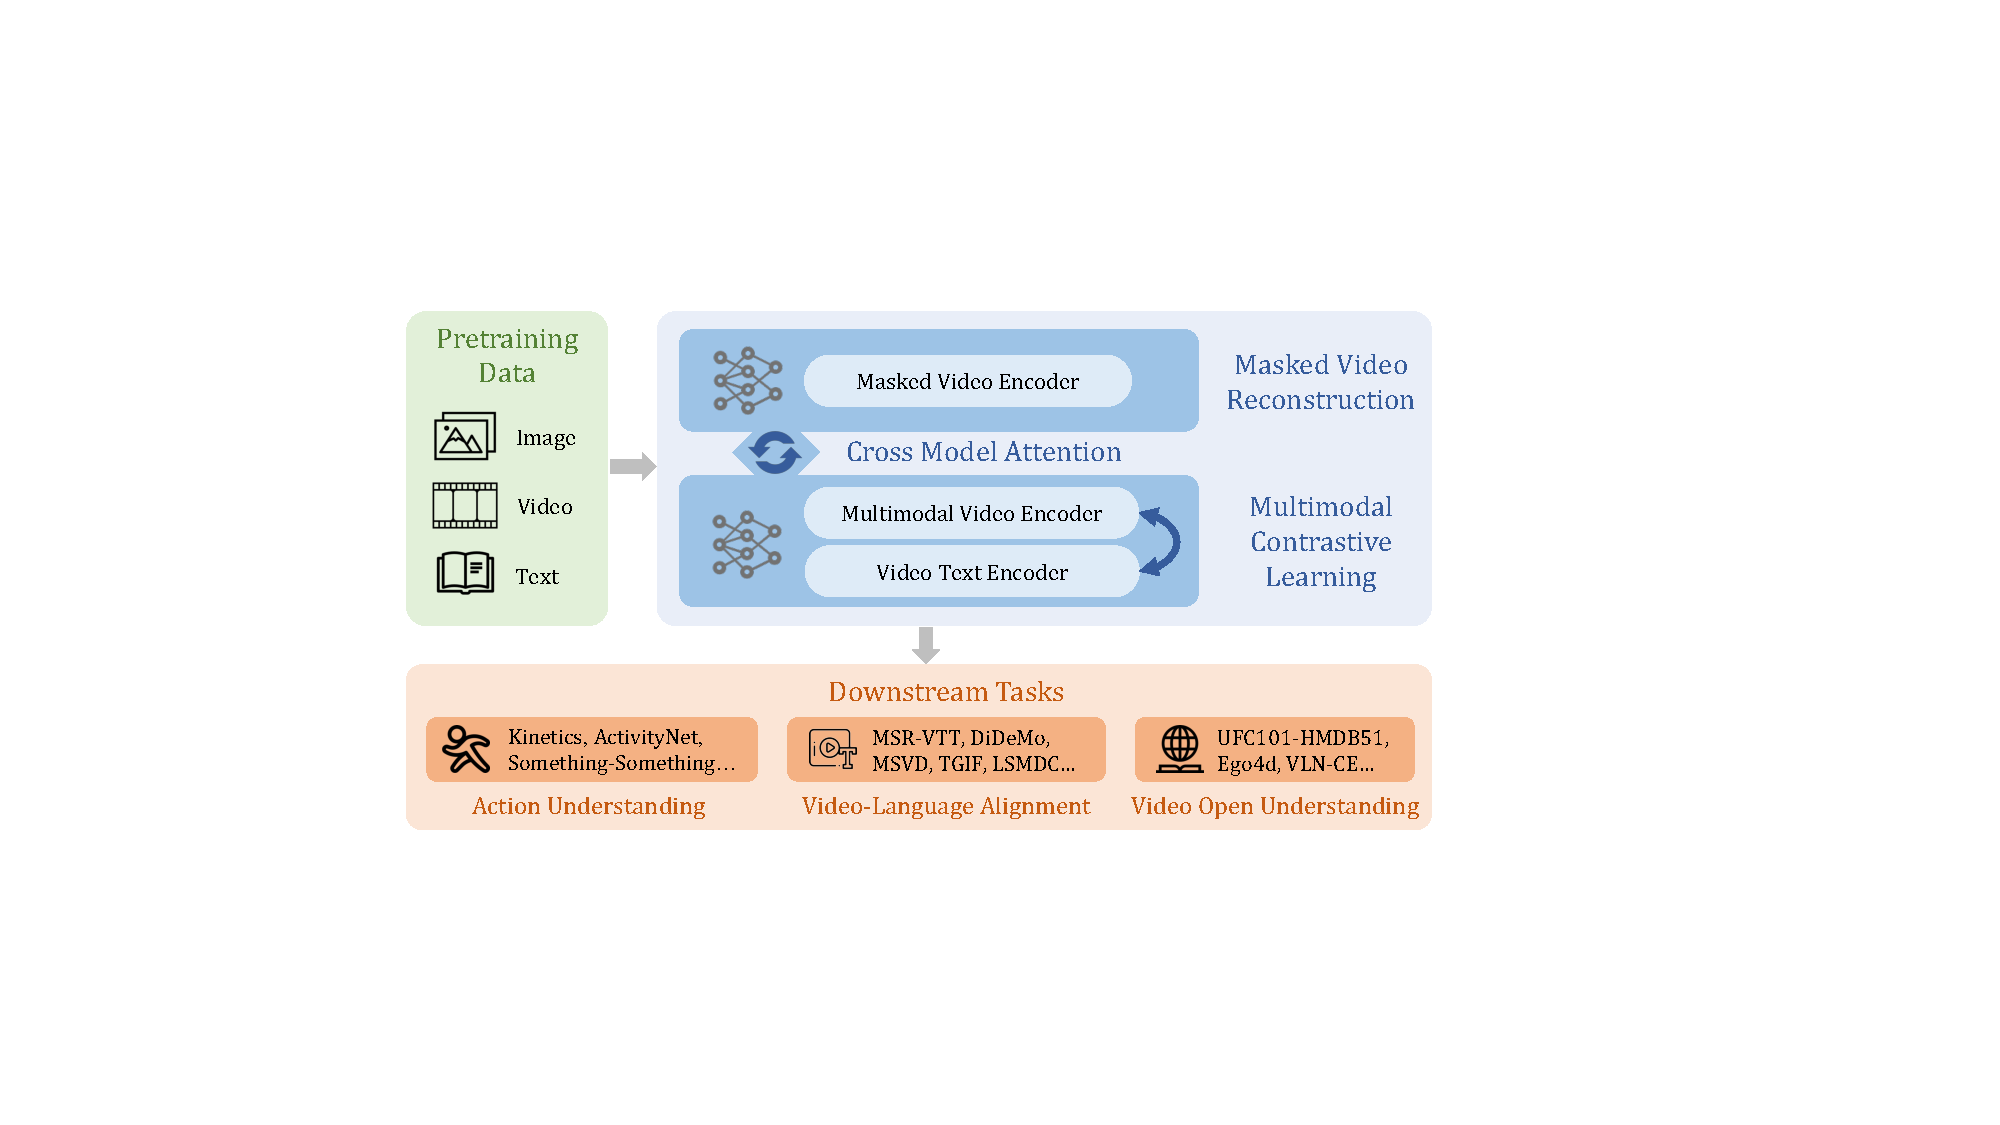
\includegraphics[width=0.9\textwidth]{content/figures/internvideo-frame3.pdf}
	\vspace{-0.3cm}
	\caption{
		The overall framework of \model.
		% Detailed explanations can be found in Section \ref{method}.
	}
	\label{frame_intern}
	\vspace{-0.6cm}
\end{figure*}
%!TeX spellcheck = en_US
%!TEX root=../main.tex
% \clearpage
% \begin{method}
	
	\section{InternVideo}
	
	\model~is a general video foundation model along with its training and internal cooperation as given in Figure \ref{frame_intern}. In structure, \model~adopts the vision transformer (ViT) \cite{dosovitskiy2020image} and its variant UniformerV2 \cite{uniformerv2}, along with extra local spatiotemporal modeling modules for multi-level representation interaction. In learning, \model~improve its representation progressively, integrating both self-supervised (masked modeling and multimodal learning) and supervised training. Moreover, as we explore two types of self-supervised learning, we further integrate their merits. \model~dynamically derives new features from these two transformers via learnable interactions, getting the best of both worlds from generative and contrastive pertaining. Through the newly aggregated features, \model~sets new performance records on 34 benchmarks from 10 mainstream video tasks, and wins championships of five tracks in recent Ego4D competitions \cite{chen2022ego4d}.
	
	
	\subsection{Self-Supervised Video Pretraining}
	
	\model~conducts both masked and contrastive training without supervision for representation learning. According to \cite{videomae,CLIP}, video masked modeling produces features that excel at action discrimination, \eg, action recognition and temporal action localization, and video-language contrastive learning is able to understand videos with semantics from text without annotations. We employ two transformers with different structures for better leveraging these two optimization targets. The final representation is constructed by adaptively aggregating these two types of representations.
	
	\subsubsection{Video Masked Modeling}
	
	We follow most rituals from our proposed VideoMAE \cite{videomae} work to train a vanilla Vision Transformer (ViT) as a video encoder for spatiotemporal modeling, as given in Figure \ref{fig:framework} (a). VideoMAE conducts a video reconstruction task with highly masked video inputs, using an asymmetric encoder-decoder architecture. The used encoder and decoder are both ViTs. The channel number of the decoder is half of that of the encoder, with 4 blocks by default. Specifically, we divide the temporal strided downsampled video inputs into non-overlapping 3D patches and project them linearly into cube embeddings. Then we apply tube masking with notably high ratios (e.g. 90\%) to these embeddings and input them into the asymmetric encoder-decoder architecture to perform the masked video modeling pretraining. To characterize spatiotemporal interaction globally, we employ joint space-time attention \cite{arnab2021vivit,liu2022video} in ViT, making all visible tokens globally interact with each other. It is computationally tractable as only a few tokens are preserved for calculation. %More details about architecture and masking are given in Supp.
	
	
	\subsubsection{Video-Language Contrastive Learning}
	
	We conduct both video/image-text contrastive learning and video captioning tasks for pretraining, as given in Figure \ref{fig:framework} (b). 
	For training efficiency,
	we build our multimodal structure based on the pretrained CLIP \cite{CLIP}. Instead of directly employing a vanilla ViT, we use our proposed UniformerV2~\citep{uniformerv2}  as the video encoder for better and more efficient temporal modeling. Moreover, we adopt an extra transformer decoder for cross-modal learning. 
	Specifically, we follow a typical align-before-fuse paradigm as given in \cite{coca,li2021align}. 
	First, video and text are separately encoded. Then a contrastive loss is utilized to align the embedding space of video and text features. In the fusing stage, we apply a caption decoder as a cross-modality fuser, which uses cross attention for a captioning pretext. This align-before-fuse paradigm not only ensures the modalities can be aligned into the same single embedding space, which is beneficial for tasks like retrieval but also gifts the model with the ability to combine different modalities and can be beneficial for tasks like question answering. The introduction of a caption decoder both extends the potential of the original CLIP and improves the robustness of multimodality features.
	
	\begin{figure*}[t]
		\centering
		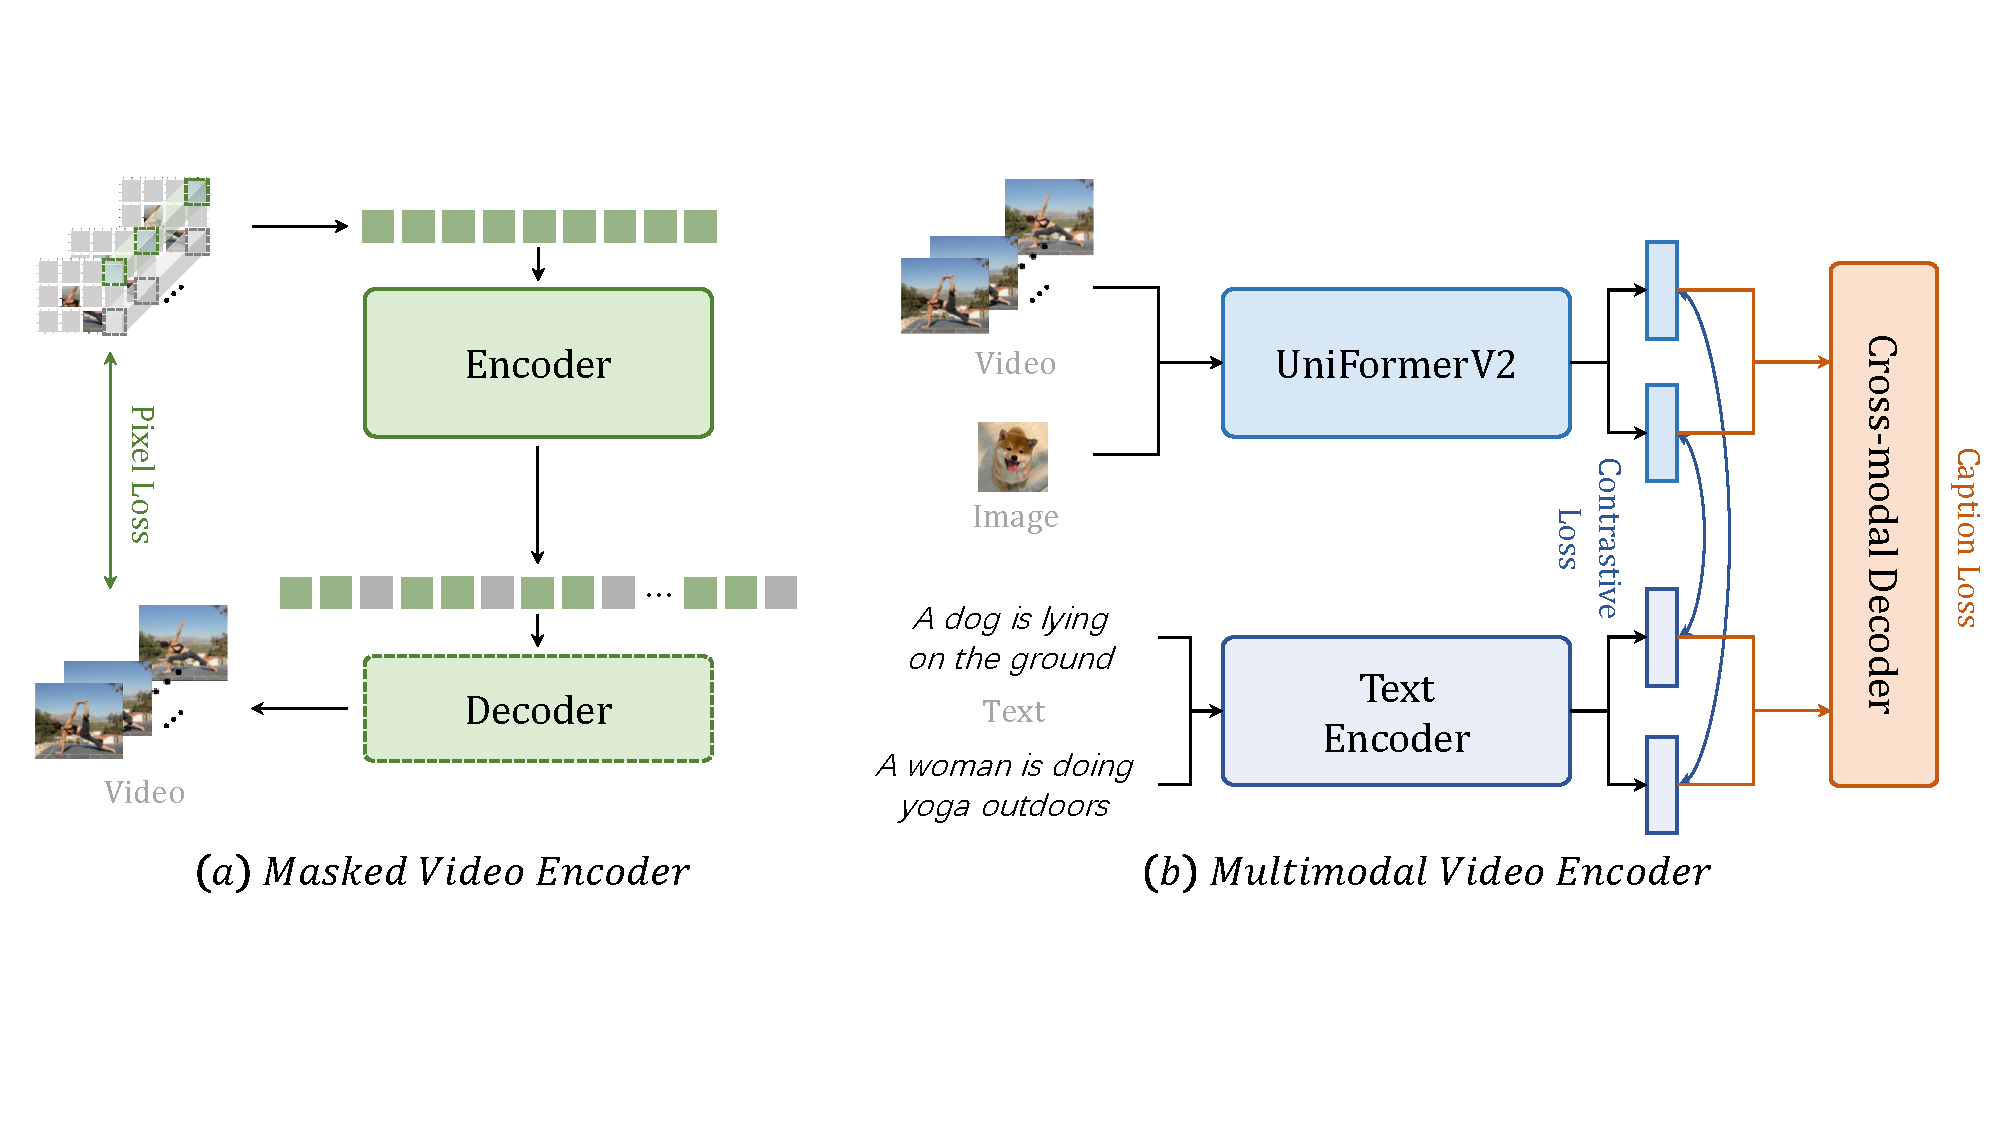
\includegraphics[width=0.9\textwidth]{content/figures/two-schemes-v2.pdf}
		\vspace{-0.1cm}
		\caption{
			The overall framework of masked learning and multimodal learning in the pretrained stage.
		}
		\label{fig:framework}
		%    \vspace{-0.4cm}
	\end{figure*}
	
	\subsection{Supervised Video Post-Pretraining}
	
	Empirically, action recognition acts well as a meta task in video downstream applications, widely validated in \cite{lin2018bsn,lin2019bmn}. Thus we train a masked video encoder and a multimodal one with supervised action classification separately as a post-pretraining step for better performance in diverse tasks. To promote the learning capacity of these encoders, we propose a unified video benchmark Kinetics-710~(K710, described in Section \ref{k710}) for finetuning our video encoders.
	
	\textbf{Masked Video Encoder.} We finetune the masked video encoder with 32 GPUs on K710. We adjust the learning rate linearly according to the base learning rate and batch size, $\textit{lr} = \textit{base learning rate} \times \frac{\textit{batch size}}{256} $. We adopt DeepSpeed\footnote{\url{https://github.com/microsoft/DeepSpeed}} framework to save memory usage and speed up training. We set the base learning rate to $0.001$, the drop path rate to $0.2$, the head dropout rate to $0.5$, the repeated sampling\cite{Hoffer2020AugmentYB} to 2, the layer decay to $0.8$, and trained for $40$ epochs.
	
	
	\textbf{Multimodal Video Encoder.}
	We follow most of the training recipes in UniFormer \cite{li2022uniformer}. For the best result, we adopt CLIP-ViT \cite{CLIP} as the backbone by default, due to its robust representation pretrained by vision-language contrastive learning.
	We insert the global UniBlocks in the last 4 layers of ViT-B/L to perform the multi-stage fusion.
	We set the base learning rate to $ 1e -5 $, the repeated sampling to 1, the batch size to 512, and trained for 40 epochs. We adopt sparse sampling \citep{wang2016temporal} with a resolution of 224 for all the datasets.
	In post-pretraining, we use a UniformerV2~\cite{uniformerv2} as the visual encoder and initialize additional parameters in a way that the output is identical to the original CLIP model which we find to be essential for good zero-shot performance. The video captioning module is a standard 6-layer transformer decoder with $c=768$ followed by a two-layer MLP. Other setting leaves CLIP Large/14 untouched. 
	
	\begin{figure*}[t]
		\centering
		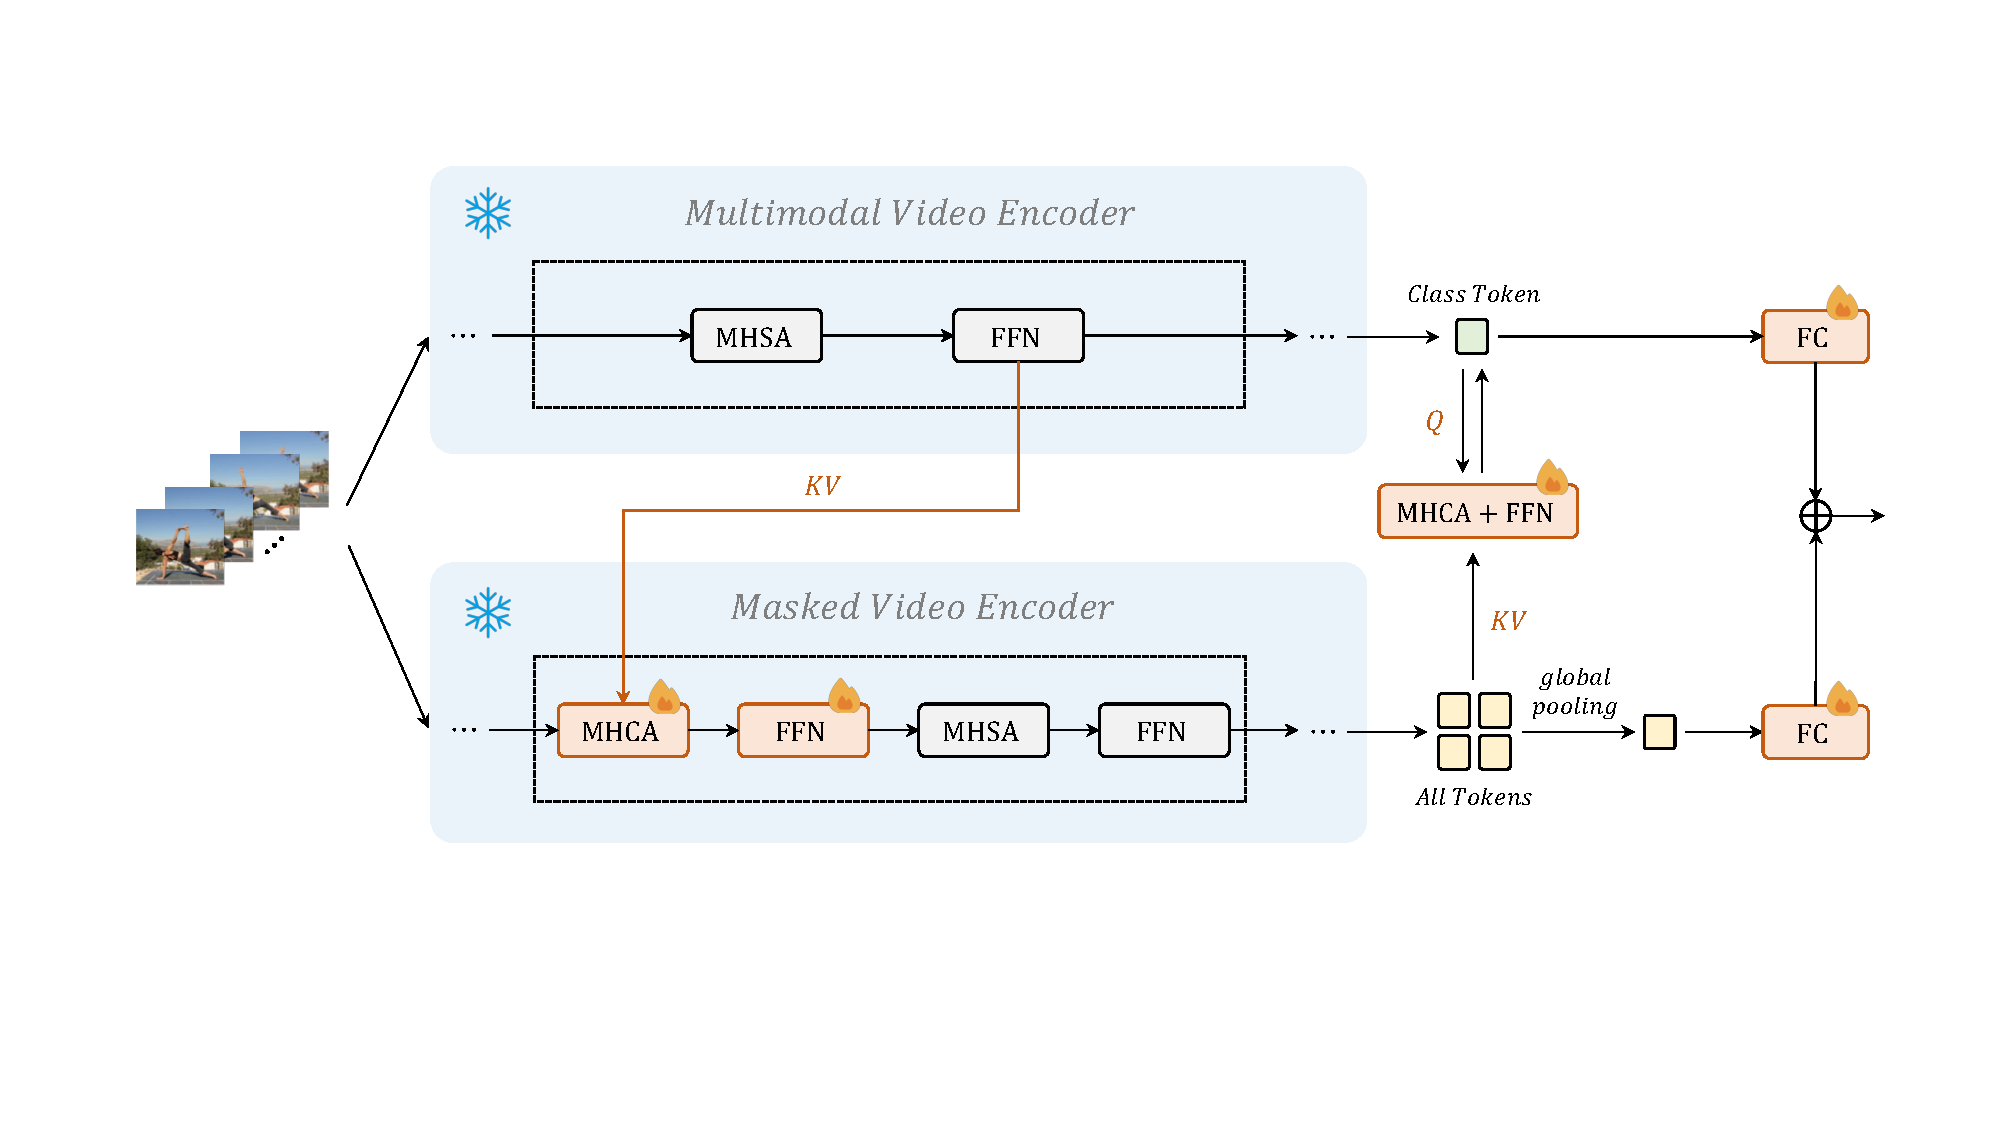
\includegraphics[width=0.9\textwidth]{content/figures/ensemble.pdf}
		\vspace{-0.1cm}
		\caption{
			The illustration of the model interaction using cross-model attention.
		}
		\label{fig:ensemble}
		\vspace{-0.4cm}
	\end{figure*}
	
	\subsection{Cross-Model Interaction}
	
	To learn a unified video representation based on both video masked modeling and video-language contrastive learning, we conduct cross-representation learning with added cross-model attention modules, as shown in Figure \ref{fig:ensemble}. 
	
	Regarding optimizing both models at the same time is computing-intensive, 
	we freeze both backbones except the classification layers and the query tokens in the multimodal video encoder, only updating newly added components.
	We add some elaborate learnable modules (cross-model attention) for aligning representations learned in different approaches. Cross-model attention (CMA) is formed by standard Multi-Head Cross Attention (MHCA) along with Feed-Forward Network (FFN). It employs intermediate tokens from a multimodal video encoder as keys and values while using these from a masked video encoder as queries. The new tokens computed from CMA are treated as a gradually aligned representation with that from the multimodal video encoder. This procedure mainly transfers multimodal knowledge to CMAs in the masked video encoder. One design exception is that for the last CMA module, its keys and values are from the tokens of the masked video encoder and the query is from the class token of the multimodal video encoder. Thus, the class token is updated based on tokens from the masked encoder. It transfers single-modal knowledge to CMA in the multimodal video encoder. From this perspective, the features in all stages of the masked video encoder and the ones in the final stage of the multimodal video encoder are enhanced to coordinate with each other, in the supervision by action recognition. Finally, we utilize a learnable linear combination to dynamically fuse the two prediction scores.
	
